\documentclass[12pt, letterpaper]{article}
\usepackage[margin=1in]{geometry}
\usepackage{tkz-euclide}
\usepackage{amsmath}
\usepackage{amssymb}
\usepackage{fancyhdr}
\usepackage{pgfplots}
\usepackage{makecell}
\usetikzlibrary{decorations.pathmorphing, patterns}
\pgfplotsset{compat=newest}
\pgfplotsdefinecstransform{polarrad along x}{cart}{%
    % First, swap axis such that we can apply polarrad->cart.
    % Note that polarrad expects (<angle>,<radius>,Z):
    \pgfkeysgetvalue{/data point/x}\X
    \pgfkeysgetvalue{/data point/y}\Y
    \pgfkeyslet{/data point/y}\X
    \pgfkeyslet{/data point/x}\Y
    \pgfplotsaxistransformcs
        {polarrad}
        {cart}%
    %
    % Ok, now we have cartesian. Swap axes such that we have them
    % along X:
    \pgfkeysgetvalue{/data point/x}\X
    \pgfkeysgetvalue{/data point/y}\Y
    \pgfkeysgetvalue{/data point/z}\Z
    \pgfkeyslet{/data point/y}\X
    \pgfkeyslet{/data point/z}\Y
    \pgfkeyslet{/data point/x}\Z
}%

\renewcommand\cellgape{\Gape[4pt]}

\title{Math-1730 Formula Sheet}
\author{Edward Nafornita \\
\small Evan Petrimoulx}

\pagestyle{fancy}
\renewcommand{\headrulewidth}{0pt}
\renewcommand{\footrulewidth}{0pt}

\fancyhf{}
\rfoot{Page \thepage}

\begin{document}
    \newcommand{\pythagwidth}{3cm}
    \newcommand{\pythagheight}{2cm}
    \maketitle{}
    \section{\underline{Indefinite Integrals:}}
        \textnormal{\textbf{Constant Integration:}}
    \begin{flalign*}
        &\int a \,dx = x + C & &\int af(x) \,dx = f(x) + C &\\
    \end{flalign*}
        \textnormal{\textbf{Distribution:}}
    \begin{flalign*}
        &\int f(x) \pm g(x) \,dx = \int f(x) \,dx \pm \int g(x) \,dx &\\
    \end{flalign*}
        \textnormal{\textbf{Exponentials:}}
    \begin{flalign*}
        &\int x^n \,dx = \frac{x^n+1}{n+1} + C, \hspace{10pt} if \hspace{5pt} n \neq -1 &
        &\int a^x \,dx = \frac{a^x}{\ln a} + C &\\
        &\int e^x \,dx = e^x + C &
        &\int \frac{1}{x} \,dx = \ln |x| + C&\\
    \end{flalign*}
        \textnormal{\textbf{Trigonometric:}}
    \begin{flalign*}
        &\int \sin x \,dx = - \cos x + C &
        &\int \cos x \,dx = \sin x + C &\\
        &\int \sec ^2x \,dx = \tan x + C &
        &\int \csc ^2x \,dx = - \cot x + C &\\
        &\int \sec x \tan x \,dx = \sec x + C &
        &\int \csc x \cot x \,dx = - \csc x + C &\\
        &\int \tan x \,dx = \ln |\sec x| + C &
        &\int \cot x \,dx = \ln |\sin x| + C &\\
        &\int \sec x \,dx = \ln |\sec x + \tan x| + C &
        &\int \csc x \,dx = \ln |\csc x - \cot x| + C &\\
        &\int \frac{1}{x^2+1} \,dx = \arctan{x} + C &
        &\int \frac{1}{\sqrt{1-x^2}} = \arcsin{x} + C &\\
    \end{flalign*}
        \text{Generalization:}\hspace{163pt}\text{Generalization:}
    \begin{flalign*}
        &\int \frac{1}{x^2+a^2} \,dx = \frac{1}{a} \arctan{\frac{x}{a}} + C, \hspace{10pt} if \hspace{5pt} a \neq 0 &
        &\int \frac{1}{\sqrt{a^2-x^2}} \,dx = \arcsin{\frac{x}{a}} + C, \hspace{10pt} if \hspace{5pt} a \neq 0 &\\
    \end{flalign*}
    \section*{\underline{Integration By Parts:}}
        \textnormal{\textbf{Formula:}}
    \begin{align}
        &\int f(x)g'(x) \,dx = f(x)g(x) - \int f'(x)g(x) \,dx &
    \end{align}
        \textnormal{Examples:}
    \begin{flalign*}
        \int x \cos x \,dx &= \int x(\sin x)' \,dx &\\
        &= x(\sin x) - \int (x)'\sin x \,dx \\
        &= x(\sin x) - \int \sin x \,dx \\
        &= x\sin x + \cos x + C \\
    \end{flalign*}
    \begin{flalign*}
        \int 2^xx \,dx &= \int x\bigg(\frac{2^x}{\ln 2}\bigg)' \,dx &\\
        &= x\frac{2^x}{\ln 2} - \int (x)'\bigg(\frac{2^x}{\ln 2}\bigg) \,dx \\
        &= x\frac{2^x}{\ln 2} - \int \frac{2^x}{ln 2} \,dx \\
        &= x\frac{2^x}{\ln 2} - \frac{1}{\ln 2}\int 2^x \,dx \\
        &= x\frac{2^x}{\ln 2} - \frac{1}{\ln 2}\cdot\frac{2^x}{\ln 2} + C\\
        &= x\frac{2^x}{\ln 2} - \frac{2^x}{\ln ^2(2)} + C\\
    \end{flalign*}
    \newpage
    \section*{\underline{U-Substitution:}}
        \textnormal{\textbf{Formula:}}
    \begin{align}
        &u = g(x)\hspace{10pt} then, &\\
        &\int f(g(x))g'(x) \,dx = \int f(u) \,du
    \end{align}
    \textnormal{When using U-Substitution, normally pick the most complex part of the problem then \\calculate "du=g'(x)" and algebraicially solve for 'dx', or until everything is in terms of 'u' and 'du'.
    }
    \textnormal{\newline\newline Examples:}
    \begin{flalign*}
        &\int x^2\cos(x^3)\,dx &\\
        &let\hspace{10pt} u=x^3 \hspace{10pt}then,\hspace{5pt} du=3x^2\,dx\\
        &\int x^2\cos(x^3)\,dx\hspace{10pt}\hspace{5pt}Sub: \cos(x^3)=\cos(u) &\\
        &\int \cos(x^3)x^2\,dx = \int \cos(u)\cdot\bigg(\frac{1}{3}\,du\bigg) &\\
        &=\int\frac{1}{3}\cos(u)\,du \\
        &=\frac{1}{3}\int\cos(u)\,dx \\
        &=\frac{1}{3}\cdot\sin(u)+C \\
        &=\frac{\sin(x^3)}{3}+C &\\
    \end{flalign*}
    \newpage
    \section*{\underline{Trionometric Integrals:}}
        \textnormal{\textbf{Formulas:}}
    \textnormal{\newline\newline\textbf{1. Integrals of the form:} \\
        $$\int\sin^m(x)\cos^n(x)\,dx$$ \\
    }
    \textnormal{\textbf{Three Cases:}\\}
    \begin{description}
        \item 1. If n is odd, save a factor of $\cos(x)$ and use $\cos^2(x)=1-\sin^2(x)$ to get everything in terms of $\sin(x)$.
        \item 2. If m is odd, save one factor of $\sin(x)$ and use $\sin^2(x)=1-\cos^2(x)$ to get everything in terms of $\cos(x)$.
        \item 3. If m, n are both even use half-angle formulas: $\sin^2(x)=\frac{1-\cos(2x)}{2}$\hspace{10pt}:\hspace{10pt}$\cos^2(x)=\frac{1+\cos(2x)}{2}$.
    \end{description}
    \textnormal{\textbf{2. Integrals of the form:} \\
        $$\int\tan^m(x)\sec^n(x)\,dx$$ \\
    }
    \textnormal{\textbf{Two Cases:}}
    \begin{description}
        \item 1. If n is even, save a factor of $\sec^2(x)$ and use $\sec^2(x)=1+\tan^2(x)$ to get everything in temrs of $\tan(x)$.
        \item 2. If m is odd, save a factor of $\sec(x)\tan(x)$ and use $\tan^2(x)=\sec^2(x)-1$ to get everything in terms of $\sec(x)$.
    \end{description}
    \textnormal{\textbf{3. Integrals of the form:}}
    \begin{description}
        \item 1. $\sin(mx)\cos(nx)\,dx$\newline Use identity: $\sin(A)\cos(B)=\frac{1}{2}\big(\sin(A-B)+\sin(A+B)\big)$
        \item 2. $\sin(mx)\sin(nx)\,dx$\newline Use identity: $\frac{1}{2}\big(\cos(A-B)-\cos(A+B))$
        \item 3. $\cos(mx)\cos(nx)\,dx$\newline Use identity: $\frac{1}{2}\big(\cos(A-B)+\cos(A+B))$
    \end{description}
    \newpage
    \subsection*{\textbf{Trigonometric Substitution:}}
    \textnormal{Idea of Trigonometric Substitution:\\
        Use the 'reverse' substitution rule in the form $x=ab(c)$, where 'a' is a suitable constant, and 'b(c)' is a suitable trigonometric function, to boil down the integral to some sort of trigonometric integral.
    }
    \newline\newline
    \begin{center}
        \begin{tabular}{|l|l|l|}
            \hline If You See & Try Subbing & This Identity will Help \\
            \hline $\sqrt{a^2-x^2}$ & \makecell{$x=a\sin(\theta)$ \\ $-\frac{\pi}{2}\leq\theta\leq\frac{\pi}{2}$} & $1-\sin^2(\theta)=\cos^2(\theta)$ \\
            \hline $\sqrt{a^2+x^2}$ & \makecell{$x=a\tan(\theta)$ \\ $-\frac{\pi}{2}<\theta<\frac{\pi}{2}$} & $1+\tan^2(\theta)=\sec^2(\theta)$\\
            \hline $\sqrt{x^2-a^2}$ & \makecell{$x=a\sec(\theta)$ \\ $0\leq\theta<\frac{\pi}{2}$ or \\ $\pi\leq\theta<\frac{3\pi}{2}$} & $\sec^2(\theta)-1=\tan^2(\theta)$\\
            \hline
        \end{tabular}
    \end{center}
    \textnormal{\newline\textbf{Examples:}}
    \begin{flushleft}
        \text{1.}\hspace{10pt}$\int x\sqrt{16-x^2}\,dx$\\
        \text{Let}\hspace{5pt}$x=4\sin(\theta),\hspace{5pt}$ \text{where}\hspace{5pt} $-\frac{\pi}{2}\leq\theta\leq\frac{\pi}{2}$,\hspace{5pt} \text{and}\hspace{5pt} $dx=4\cos(\theta)\,d\theta.$\\
        $\sqrt{16-x^2} = \sqrt{16-(4\sin(\theta)^2} $\\
        \hspace{51pt}= $\sqrt{16-16\sin^2(\theta)}$ \\
        \hspace{51pt}= $\sqrt{16(1-\sin^2(\theta))}$ \\
        \hspace{51pt}= $\sqrt{16(\cos^2(\theta))}$ \\
        \hspace{51pt}= $|4\cos(\theta)|$ \\
        \hspace{51pt}= $4\cos(\theta)$ because $4\cos(\theta)\geq0$ for $-\frac{\pi}{2}\leq\theta\leq\frac{\pi}{2}$.\\
        $\int x\sqrt{16-x^2}\,dx = \int(4\sin(\theta)\cdot(4\cos(\theta))\cdot(4\cos(\theta))\,d\theta$ \\
        \hspace{83pt}= $64\int\sin(\theta)\cos^2(\theta)\,d\theta$ \\
        Let $u=\cos(\theta)$, $du=-\sin(\theta)\,d\theta$. \\
        \hspace{83pt}= $-64\int u^2\,du$ \\
        \hspace{83pt}= $-64\cdot\frac{u^3}{3}+C$ \\
        \hspace{83pt}= $-\frac{64}{3}\cos^3(\theta)+C$ \\
    \end{flushleft}
    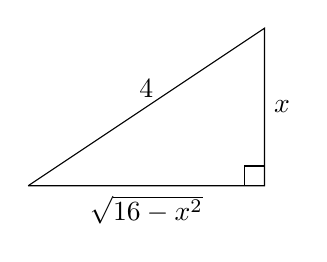
\begin{tikzpicture}[scale=1.00]
        \coordinate (C) at (-1.5cm,-1.cm);
        \coordinate (A) at (1.5cm,-1.0cm);
        \coordinate (B) at (1.5cm,1.0cm);
        \draw (C) -- node[above] {$4$} (B) -- node[right] {$x$} (A) -- node[below] {$\sqrt{16-x^2}$} (C);
        \draw (1.25cm,-1.0cm) rectangle (1.5cm,-0.75cm);
    \end{tikzpicture}
    \begin{flushleft}
        By Pythagorean Theorem:
        $\cos(\theta)=\frac{\sqrt{16-x^2}}{4}$ \\
        $\int x\sqrt{16-x^2}\,dx=-\frac{64}{3}\cdot\frac{\sqrt{16-x^2}^3}{4^3}+C$\\
        $\int x\sqrt{16-x^2}\,dx=-\frac{\sqrt{16-x^2}^3}{3}+C$\\
    \end{flushleft}
    \newpage
    \section*{\underline{Partial Fraction Decomposition:}}
    \begin{description}
        \item Case 1: Q(x) is a product of distinct linear factors \\ $Q(x)=(a_1x+b_1)(a_2x+b_2)+\dots(a_kx+b_k)$ \\ The partial fraction decomposition of f(x) is $\frac{P(x)}{Q(x)}=\frac{A_1}{a_1x+b_1}+\frac{A_2}{a_2x+b_2}+\dots+\frac{A_k}{a_kx+b_k}$.
        \item Case 2: Q(x) is a product of linear factors, some of which are repeated. If $(a_ix+b_i)^r$ \\ (where r $\neq$ 1) occurs in the factorization of Q(x) then instead of $\frac{A_i}{a_ix+b_i}$ term, we will have the sum: $\big(\frac{B_1}{a_ix+b_i}+\frac{B_2}{a_ix+b_i}^2+\dots+\frac{B_i}{a_ix+b_i}^i\big)\epsilon\mathbb{R}$.
        \item Case 3: If Q(x) has a non-repeated quadratic factor $ax^2+bx+c$, then there is a $\frac{Ax+B}{ax^2+bx+c}$ term. 
        \item Case 4: More generally, if Q(x) has a repeated quadratic factor $ax^2+bx+c$, then you will see: $\frac{A_1x+B_1}{ax^2+bx+c}+\frac{A_2x+B_2}{ax^2+bx+c}^2+\dots+\frac{A_rx+B_r}{ax^2+bx+c}^r$
    \end{description}
    \textnormal{\textbf{Examples:}}
    \begin{flushleft}
        $$\int\frac{x}{x^2+4x+3}\,dx$$
        Factor $x^2+4x+3=(x+3)(x+1)$\\
        Then the form of the partial fraction decomposition is:$$\frac{x}{(x+1)(x+3)}=\frac{A}{x+1}+\frac{B}{x+3}$$\\
        Reduce the fractions: $\frac{x}{(x+1)(x+3)}=\frac{A}{x+1}+\frac{B}{x+3}\mid\cdot(x+1)(x+3)$\\
        $x=A(x+3)+B(x+1)$, is true $\forall x\epsilon\mathbb{R}$. \\
        Let $x=-3$\\
        $-3=A(-3+3)+B(-3+1)$\\
        $-3=-2B$\\
        $B=\frac{3}{2}$\\
        Let $x=-1$ \\
        $-1=A(-1+3)+B(-1+1)$\\
        $-1=2A$\\
        $A=-\frac{1}{2}$\\
        $\int\frac{x}{x^2+4x+3}\,dx=\int\big(\frac{-\frac{1}{2}}{x+1}+\frac{\frac{3}{2}}{x+3}\big)\,dx$\\
        \hspace{66pt}=$-\frac{1}{2}\ln|x+1|+\frac{3}{2}\ln|x+3|+C$\\
    \end{flushleft}
    \newpage
    \section{\underline{Definite Integrals:}}
        \textnormal{\textbf{Formula:}}
    \begin{equation}
        \int_a^bf(x)\,dx=F(b)-F(a)
    \end{equation}
    \begin{flushleft}
        \textbf{Examples:}\\
        $$\int_0^1x^2\,dx=\frac{x^3}{3}\bigg|_0^1=\frac{1^3}{3}-\frac{0^3}{3}=\frac{1}{3}$$
        In Essence: Compute the indefinite integral first, then apply the definite integral formula. \\
    \end{flushleft}
    \subsection*{Properties of Definite Integrals}
    \begin{description}
        \item 1. $\int_a^af(x)\,dx=0$
        \item 2. $\int_b^af(x)\,dx=-\int_a^bf(x)\,dx$
        \item 3. $\int_a^bf(x)\,dx+\int_b^cf(x)\,dx=\int_a^cf(x)\,dx$
    \end{description}
    \subsection*{Improper Integrals}
    \begin{tikzpicture}
        \begin{axis}[axis lines = middle, xlabel = \(x\), ylabel = \(y\)]
            \addplot [
                domain=-10:10, 
                samples = 50, 
                color = blue,
                ]
                {1/x^2};
            \addlegendentry{\(y=1/x^2\)}
        \end{axis}
    \end{tikzpicture}
    \begin{flushleft}
        The area below this graph can be denoted as $A(t)=\int_1^t\frac{1}{x^2}\,dx$, and the solution would be: $\int_1^t\frac{1}{x^2}\,dx=-\frac{1}{x}\big|_1^t=-\frac{1}{t}-(-\frac{1}{1})=1-\frac{1}{t}$\\
        Therefore, to calculate this improper integral, we must take the limit and see where it approaches.\\
        $A=\lim_{t \to \infty}A(t)=\lim_{t \to \infty}(1-\frac{1}{t})=1$\\
    \end{flushleft}
    \newpage
    \begin{flushleft}\textbf{First Type of Improper Integrals:}\end{flushleft}
    \begin{description}
        \item 1: If $\int_a^tf(x)\,dx$ is defined for all $t\geq a$, define\\$\int_a^\infty f(x)\,dx=\lim_{t \to \infty}\int_a^tf(x)\,dx$, if the limit exists, the integral is convergent, otherwise, it's divergent.
        \item 2: If $\int_t^bf(x)\,dx$ is defined for all $t\leq b$, define\\$\int_{-\infty}^bf(x)\,dx=\lim_{t \to -\infty}\int_t^bf(x)\,dx$.
        \item 3: If $\int_a^\infty f(x)\,dx$ and $\int_{-\infty}^af(x)\,dx$ converge, let\\$\int_{-\infty}^\infty f(x)\,dx=\int_a^\infty f(x)\,dx+\int_{-\infty}^af(x)\,dx$
    \end{description}
    \begin{flushleft}
        \textbf{Examples:}\\
        $$1. \int_1^\infty\frac{1}{x}\,dx=\lim_{t \to \infty}\int_1^t\frac{1}{x}\,dx=\lim_{t \to \infty}(\ln|x|\big|_1^t)=\lim_{t \to \infty}\ln(t)-\ln(1)=\lim_{t \to \infty}ln(t)=+\infty$$\\
        Since $\int_1^\infty \frac{1}{x}\,dx$ is not finite (meaning doesn't resolve to an approachable number), therefore $\int_1^\infty \frac{1}{x}\,dx$ diverges.
    \end{flushleft}
    \begin{flushleft}\textbf{Second Type of Improper Integrals:}\end{flushleft}
    \begin{description}
        \item 1: If f(x) is continuous on [a,b) and discontinuous at b, define\\$\int_a^bf(x)\,dx=\lim_{t \to b^-}\int_a^tf(x)\,dx$.
        \item 2: If f(x) is continuous on (a,b] and discontinuous at a, define\\$\int_a^bf(x)\,dx=\lim_{t \to a^+}\int_t^bf(x)\,dx$.
        \item 3: If f(x) has a discontinuity at c$\epsilon$(a,b) and $\int_a^cf(x)\,dx$ and $\int_c^bf(x)\,dx$ converges, define\\$\int_a^bf(x)\,dx=\int_a^cf(x)\,dx+\int_c^bf(x)\,dx$.
    \end{description}
    \begin{flushleft}
        \textbf{Examples:}\\
        $1. \int_0^1\frac{1}{\sqrt{x}}\,dx$, is an improper integral since it's discontinuous at x=0.\\
        $$\int_0^1\frac{1}{\sqrt{x}}\,dx=\lim_{t \to 0^+}\int_t^1\frac{1}{\sqrt{x}}\,dx=\lim_{t \to 0^+}\frac{x^{\frac{1}{2}}}{\frac{1}{2}}\bigg|_t^1=\lim_{t \to 0^+}\bigg(\frac{1^{\frac{1}{2}}}{\frac{1}{2}}-\frac{t^{\frac{1}{2}}}{\frac{1}{2}}\bigg)=\frac{\frac{1}{1}}{2}=2$$\\
        Since $\int_0^1\frac{1}{\sqrt{x}}\,dx$ is finite (meaning it does resolve to an approachable number), therefore $\int_0^1\frac{1}{\sqrt{x}}\,dx$ converges.
    \end{flushleft}
    \newpage
    \subsection*{Areas Between Curves:}
    \begin{flushleft}
        If $f(x)\geq g(x) \forall x\epsilon[a,b]$ then the area bounded by the curves; y=f(x), y=g(x), x=a, and x=b is $A=\int_a^b(f(x)-g(x))\,dx$.\\
    \end{flushleft}
    \textnormal{\textbf{Examples:}}
    \textnormal{\newline\newline}
    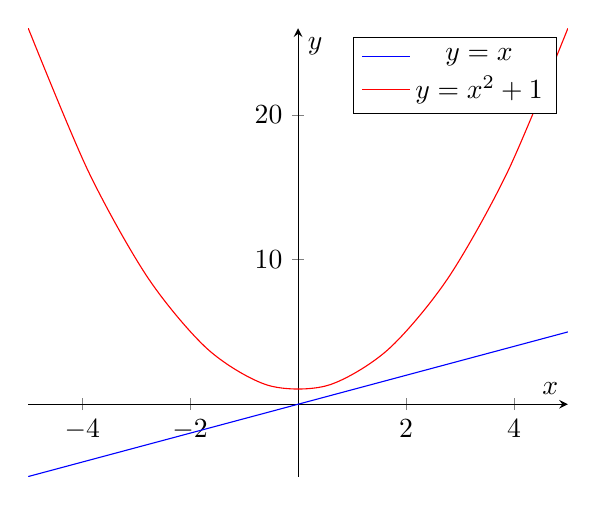
\begin{tikzpicture}
        \begin{axis}[axis lines = middle, xlabel = \(x\), ylabel = \(y\)]
            \addplot [domain = -5:5, smooth, samples = 10, color = blue,]{x};
            \addplot [domain = -5:5, smooth, samples = 10, color = red,]{x^2+1};
            \addlegendentry{\(y=x\)}
            \addlegendentry{\(y=x^2+1\)}
        \end{axis}
    \end{tikzpicture}
    \begin{flushleft}
        $$A=\int_{-1}^1(f(x)-g(x))\,dx$$\\
        Let f(x) be the bigger function; $f(x)=x^2+1$, then $g(x)=x$\\
        $$A=\int_{-1}^1(x^2+1-x)\,dx=\frac{x^3}{3}+x-\frac{x^2}{2}\bigg|_1^1=\frac{1}{3}+1-\frac{1}{2}-\bigg(-\frac{1}{3}-1+\frac{1}{2}\bigg)=\frac{2}{3}+2-1=\frac{5}{3}$$\\
    \end{flushleft}
    \newpage
    \section{\underline{Volumes Via Areas of Cross Sections:}}
    \indent If a solid lies between the planes x = a and x = b and A(x) is the area of the x-cross-section for $a<= x <= b$, then the volume of a solid is:
        \begin{equation}
            V = \int_{a}^{b} A(x) dx
        \end{equation}
    \subsection*{Example - The Volume of a Sphere of Radius R:}
    %% Insert Graph of Sphere // Circle Here %%
    \begin{equation*}
        R^2 = |x|^2 + r^2
    \end{equation*}
    Where R is the radius of the sphere, r is the length of the cross section, and |x| os the x-distance tothe slice / cross section. 
    \begin{equation*}
        r = \sqrt{R^2 - x^2}
    \end{equation*}

    \begin{equation*}
        V = \int_{-R}^{R} A(x) dx = \int_{-R}^{R} \pi (R^2 - x^2)dx
    \end{equation*}
    
    \begin{equation*}
        \pi R^2 x - \pi \frac{x^3}{3} \bigg| ^{R}_{-R} = \left(\pi R^3 - \pi \frac{R^3}{3}\right) - \left( -\pi R^3 + \pi \frac {\pi R^3}{3}\right)
    \end{equation*}
    
    \begin{equation*}
        \frac{2\pi}{3} R^3 - \left(- \frac{2\pi}{3}R^3\right) = \frac{4\pi R^3}{3}
    \end{equation*}
    
    \subsection*{Solids of Revolution}
    
    \begin{flushleft}
        There are different formats for solids of revolution:
        \begin{itemize}
            \item Cylinders
            \item Cones
            \item Tori (sing. torus)
        \end{itemize}
        Each of which have two different methods on computing them:
        \begin{itemize}
            \item Disk/Washer Method
            \item Cylindrical Shells Method
        \end{itemize}
    \end{flushleft}
    
    \section*{Disk/Washer}
        \begin{itemize}
            \item If the cross-section is a disk, then its area is
                \begin{equation}
                    A(x) = \pi(radius)^2
                \end{equation}
            \item If the cross-section is a washer (annulus), then its area is
                \begin{equation}
                    A(x) = \pi[(outer\hspace{5pt}radius)^2 - (inner\hspace{5pt}radius)^2]
                \end{equation}
        \end{itemize}
    
    \section*{Cylindrical Shells}
        Let $b > a >= 0$, $ f(x) >= 0$ on $[a, b]$ and R, the region under the graph of $y = f(x)$ betwen $x = a$ and $x = b$. The volume of the solid of revololution is obtained by rotating R around the y-axis. 
        \begin{equation}
            V = \int^b_a 2\pi x f(x) dx
        \end{equation}
        It is important to note the Surface Area of a cylindrical shell:
        \begin{equation*}
            2\pi h r
        \end{equation*}

        Idea: Slice the solid of revilution into cylindrical shells. You want to make the cylinder for every $dx$ until you can approximate the area.

        \begin{equation*}
            V = \int^b_a \left(surface \hspace{5pt} area\hspace{5pt}  of \hspace{5pt}  cylindrical\hspace{5pt} shell \right) dx
        \end{equation*}

        \begin{equation*}
            V = \int^b_a 2\pi \left( height\right) \left( radius\right) dx = \int^b_a 2\pi x f(x) dx
        \end{equation*}
        
    
    \textbf{Example:}
    \begin{center}
        \begin{tikzpicture}
            \pgfdeclareverticalshading{brighter}{100bp}{
                rgb(0bp)=(0.1,0.55,0);
                rgb(100bp)=(0.8,0.9,0)
            }
            
            \pgfdeclareverticalshading{darker}{100bp}{
                rgb(0bp)=(0.5,0.75,0);
                rgb(100bp)=(0,0.5,0)
            }
            
            \begin{axis}
                colormap/greenyellow,
                view={12}{30}]
                
                \def\generatrix{(((2*x^4)/27) - ((4*x^3)/9))}
                
                \addplot3[
                    surf,
                    shader=faceted interp,
                    samples=30,
                    domain=0:6,
                    domain y=0:3*pi/2,
                    z buffer=sort,
                    data cs=polarrad along x]
                ({\generatrix},y,x);
        
                \addplot3[
                    draw=none,
                    shading=darker,
                    fill opacity=1.0,
                    samples=30,
                    samples y=1,
                    domain=0:6,
                    data cs=polarrad along x]
                ({\generatrix},0,x) --cycle;
        
                \addplot3[
                    draw=none,
                    shading=brighter,
                    fill opacity=1.0,
                    samples=30,
                    samples y=1,
                    domain=0:6,
                    data cs=polarrad along x]
                ({\generatrix},3*pi/2,x) --cycle;
        
                \addplot3[
                    surf,
                    opacity = 0.1,
                    shader=faceted interp,
                    samples=30,
                    samples y = 10,
                    domain=0:6,
                    domain y=3*pi/2:2*pi,
                    z buffer=sort,
                    data cs=polarrad along x]
                ({\generatrix},y,x); 
            \end{axis}
        \end{tikzpicture}
    \end{center}

    \section{\underline{Physical Applications}}
    \subsection*{Work}
        If a constant force, \textit{F}, acts on an object. The work done to move the object a distance, \textit{d}, is:
        \begin{equation}
            W = F\cdot d
        \end{equation}
        If the object moves from, x = a, to x = b, under the action of a variable force, F(x), where (x) is the position, the work is:
        \begin{equation}
            W = \int_a^bF(x)\,dx
        \end{equation}
    \subsubsection*{Example}
        When a particle is x meters from the origin, a force of $F(x) = 3x^2$ Newtons acts on it. How much work is done moving it from x = 2, to x = 4?
        \begin{equation*}
            W = \int_2^4F(x)\,dx = \int_2^4 3x^2\,dx
            = x^3\big|_2^4 = 4^3 - 2^3 = 56J
        \end{equation*}
    \subsection*{Hooke's Law}
    The force required to maintain a spring stretched x-units beyond its natural length is $F=k\Delta x$ where k is the spring constant. 
    
    \subsubsection*{Example}
        A force of 60N is required to hold a spring stretched 5cm beyond its natural length. How much work is 
        done in stretching the spring 5cm beyond it's natural length (Starting from its original, natural length). From 5cm to 10cm beyond its natural length?
        
        \begin{center}
            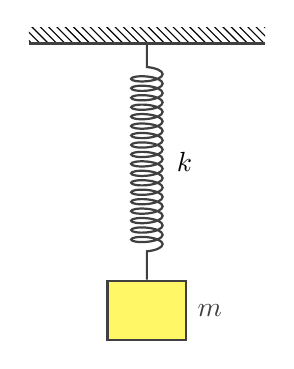
\begin{tikzpicture}[black!75,thick]
                % Supporting structure
                \fill [pattern = north west lines] (-1.5,0) rectangle ++(3,.2);
                \draw[thick] (-1.5,0) -- ++(3,0);
                 
                % Spring 
                \draw [
                    decoration={
                        coil,
                        aspect=0.3, 
                        segment length=1.2mm, 
                        amplitude=2mm, 
                        pre length=3mm,
                        post length=3mm},
                    decorate
                ] (0,0) -- ++(0,-3) node[midway,right=0.25cm,black]{$k$}; 
                 
                % Mass
                \node[draw,
                    fill=yellow!60,
                    minimum width=1cm,
                    minimum height=0.75cm,
                    anchor=north,
                    label=east:$m$] at (0,-3) {};
            \end{tikzpicture}
        \end{center}
        
        \begin{equation*}
            F = k \Delta x
        \end{equation*}
        \begin{equation*}
            60 = k(0.05m)
        \end{equation*}
        \begin{equation*}
            1200 = k
        \end{equation*}
        \begin{equation*}
            W = \int^{0.05}_0 1200x dx = 1200 \int^{0.05}_0 x dx = \frac{1200x^2}{2} \bigg|^{0.05}_0 = 600(0.05)^2 = 1.5J
        \end{equation*}
        \begin{equation*}
            W = \int^{0.1}_{0} 1200x dx = 600x^2 \bigg|^{0.1}_{0.05} = 600((0.1)^2 - (0.05)^2) = 4.5J
        \end{equation*}
        
    \subsection*{Average Values of Functions:}
        \textit{Definition}\\
        The average value of a function on the interval $[a, b]$ is:
            \begin{equation*}
                f_{ave} = \frac{1}{b - a} \int^b_a f(x) \,dx
            \end{equation*}

    \subsection*{Mean Value Theorem For Integrals}
        If f is continuous on$[a, b]$, then there exists some $c \epsilon [a, b]$ such that:
            \begin{equation*}
                f(c) = f_{ave} = \frac{1}{b-a} \int^b_a f(x) \,dx
            \end{equation*}
        The fundamental theorem of calculus implies that the mean value theorem for Integrals and the mean value theorem for Derivatives are equivalent. 

    \subsection*{Centers of Mass}
        The center of mass of n point masses $m_1, m_2, m_3, ..., m_n$ at the points $(x_1, y_1), (x_2, y_2), (x_3, y_3)...(x_n, y_n)$ is $(\bar{x}, \bar{y})$  where:
            \begin{equation*}
                \bar{x} = \frac{\sum_{i}^{n}m_i x_i}{\sum_{i}^{n}m_i}
            \end{equation*}
        and
            \begin{equation*}
                \bar{y} = \frac{\sum^n_i m_i y_i}{\sum^n_i m_i}
            \end{equation*}

        Let $f(x) >= g(x)$ and R be the region bounded by the graphs $y = f(x)$ and $y = g(x)$ between $x = a$ and $x = b$. Then the center of mass (sometimes called the centroid) of R is the point $(\bar{x}, \bar{y})$ where;
            \begin{equation*}
                \bar{x} = \frac{1}{A} \int^b_a x(f(x) - g(x)) \,dx
            \end{equation*}
            \begin{equation*}
                \bar{y} = \frac{1}{2A} \int^b_a (f(x)^2 - g(x)^2) \,dx
            \end{equation*}
        And "A" is the area of R

    \subsection*{Surface of Revolution}
        
        Translation: Surface Area of a Solid of Revolution\\
        If the curve, $y = f(x)$, $a \leq x \leq b$ (with $f'(x)$ continuous), is rotated around the x-axis, we obtain a surface of revolution whose surface area is:
        \begin{equation}
            A = \int_{a}^{2} 2 \pi f(x) \sqrt{1 + f'(x)} \,dx
        \end{equation}
        In Leibnitz notation: $A = \int_a^b 2\pi f(x) \sqrt{1 + f'(x)} \,dx$ \\
        If $x = g(y)$, $c \leq y \leq d$, then: $A = \int_a^b 2 \pi y \sqrt{1 + (\frac{dx}{dy})^2} \,dy$ \\
        If rotating around y-axis: $A = \int_a^b 2\pi x \sqrt{1 + (\frac{dy}{dx})^2} \,dx = \int_c^d 2\pi x \sqrt{1 + (\frac{dx}{dy})^2} \,dy$
    \section{\underline{Sequences}}
        In this course we will only consider infinite sequences\\
        \textit{Notation:}
            \begin{equation*}
                a_n = \frac{n}{2n-1},\hspace{5pt} n \geqslant 3 \hspace{5pt} or \hspace{5pt} \bigg\{ \frac{n}{2n-1} \bigg\} ^\infty _{n=3}
            \end{equation*}
        There are various ways to descrive a sequence:
        \begin{center}
            \begin{itemize}
                \item By formula $(a_n = 2^n$ for $n \geqslant 0)$
                \item By a recurrence relation ($a_0 = 1$ and $a_n = 2a_{n-1}$ for $n \geqslant 1$)
            \end{itemize}
        \end{center}
        
        \subsection*{Limits of Sequences (Informal Definition)}
            The sequence of $a_1$, $a_2$, ...$a_n$ has a Limit L if we can make $a_n$ as close as we want to L by making n sufficiently large. 
            \begin{equation*}
                \lim_{n \to \infty} a_n = L \hspace{10pt} or \hspace{10pt} a_n \to L
            \end{equation*}

            The sequence $a_n$ has limit L or the sequence $a_n$ tends to / approaches / converges to L\\
            If $a_n$ has a finite limit, then it is caled \underline{convergent}. If it does not, it is referred to as \underline{divergent}.
        
        \subsection*{Limits of Sequences (Rigorous)}
            The sequence $a_1 , a_2 , a_3 , ... a_n$ has limit L if any $\epsilon > 0$. There exists a positive integer N such that $|a_n - L| < \epsilon \, \forall \, n \geqslant N$.\\
            There is a notation of infinite limits $lim_{n \to \infty} a_n = +\infty$ (respectively $-\infty$) if we can make $a_n$ as large (respectively as small) as we want by making n sufficiently large. 
            The sequence $a_1$, $a_2$, ... has limit $+\infty$ if for any number M, there exists a postive integer N such that $a_n > M \, \forall \, n \geqslant N$
            
        
        \subsection*{Limit Laws For Sequences}
            If ${a_n}$ and ${b_n}$ are convergent sequences, then:
            \begin{equation*}
                \lim_{n \to \infty} (a_n + b_n) = \lim_{n \to \infty} a_n + \lim_{n \to \infty} b_n
            \end{equation*}
            \begin{equation*}
                \lim_{n \to \infty} (a_n - b_n) = \lim_{n \to \infty} a_n - \lim_{n \to \infty} b_n
            \end{equation*}
            \begin{equation*}
                \lim_{n \to \infty} ca_n = c \lim_{n \to \infty} a_n
            \end{equation*}
            \begin{equation*}
                \lim_{n \to \infty} (a_n b_n) = \lim_{n \to \infty} a_n \cdot \lim_{n \to \infty} b_n
            \end{equation*}
            \begin{equation*}
                \lim_{n \to \infty} \frac{a_n}{b_n} = \frac{\lim_{n \to \infty} a_n}{\lim_{n \to \infty} b_n} \hspace{10pt} if \hspace{5pt} \lim_{n \to \infty} \neq 0
            \end{equation*}
            
        \subsection*{Squeeze Theorem for Sequences}
            If $a_n \leq b_n \leq c_n \, \forall \, n \hspace{5pt} or \hspace{5pt} n\geq n_0 \, \exists \, n_0$
            \begin{equation*}
                \lim_{n \to \infty} a_n = \lim_{n \to \infty}c_n = L \Longrightarrow \lim_{n \to \infty}b_n = L
            \end{equation*}

            If $\lim_{n \to \infty} a_n = L$ and f is continuous at L, then:
            \begin{equation*}
                \lim_{n \to \infty} F(a_n) = f(L)
            \end{equation*}
            If f is a function such that $\lim_{x \to \infty} f(x) = L$ and $a_n = f(n)$ then:
            \begin{equation*}
                \lim_{n \to \infty} a_n = L
            \end{equation*}

            A sequence is \underline{not} convergent  if and only if:
            \begin{center}
                \begin{itemize}
                    \item It has a subsequence with limit $\pm \infty$
                    \item It has two convergent subsequences with different limits. 
                    \item Examples: $(-1)^n$, n, $(-1)^n n$
                \end{itemize}
            \end{center}
            \underline{DEFINITION}\\
            A sequence $\{a_n\}$ is increasing if $a_n < a_{n+1} \, \forall \, n$. It is decreasing if $a_n > a_{n+1} \, \forall \, n$. A sequence which is either increasing or decreasing is called a monotomic.\\
            A sequence $\{ a_n \}$ is bounded above if there exists a number M such that $a_n \leq M \, \forall \, n$. It is bounded below if there exists a number < such that $a_n \leq M \, \forall \, n$. It is bounded if it is bounded both above and below.
            
    \section{\underline{Series}}
        An (infinite) series is an infinite summation: $$a_1 + a_2 + a_3 + \cdots + a_n = \sum_{n = 1}^\infty a_n$$
        Infinite summations don't need to have a value, but some do. \\

            \subsubsection*{Definition}
                Let $\sum_{n = 1}^\infty$ be a series. The n-th partial sum is:
                \begin{equation}
                    S_n = a_1 + a_2 + a_3 + \cdots + a_n = \sum_{i=1}^n a_i
                \end{equation}
                If the sequence ${S_n}$ is convergent, then $\sum_{n=1}^\infty = S$. The number S is the sum of the series. However if the sequence is divergent, then so is the series.\\
                Note: If $\sum_{n = 1}^\infty a_n$ is convergent, then the $\lim_{n \to \infty} a_n = 0$\\
                \indent However, if $\lim_{n \to \infty} a_n = 0 \neq \sum_{n = 1}^\infty a_n$ is convergent.
        
        \subsection*{Test for Divergence}
            If ${a_n}$ is divergent or $\lim_{n \to \infty} a_n \neq 0$ then $\sum_{n = 1}^\infty a_n$ is divergent.\\
        
            Typically, it is not too hard to determine whether a series is convergent or divergent, but most of the time it is extremely hard (often impossible) to determine precisely the sum of the series if it's convergent.\\
            Some exceptions are:
        
        \subsection*{Telescoping Sums}
            Idea: Find ${b_n}$ such that $a_n = b_{n+1} - b_n$ or some variabtion on this idea (eg. $a_n = b_{n+k} - b_n$ where k is a constant, or anything that leads up to a massive simplification when summing up).
            \subsubsection*{Example:}
                $$\sum_{n = 1}^\infty \frac{1}{n(n+1)} = \frac{1}{1\cdot 2} + \frac{1}{2\cdot 3} + \frac{1}{3\cdot 4} + \dots$$
                Solution: The n-th partial sum is,
                \begin{equation*}
                    S_n = \frac{1}{1\cdot 2} + \frac{1}{2\cdot 3} + \dots + \frac{1}{n(n+1)} = \sum_{i = 1}^n \frac{1}{i(i+1)}
                \end{equation*}
                \begin{flalign*}
                    \sum_{n = 1}^n \frac{1 + i - i}{i(i + 1)} &= \sum_{i = 1}^n \frac{(i + 1)}{i(i + 1)} - \frac{i}{i(i+1)} \\
                    &= \sum_{i = 1}^n (\frac{1}{i} - \frac{1}{i + 1})\\ &= 1 - \frac{1}{n + 1} \\
                    \lim_{n \to \infty} S_n = \lim_{n \to \infty} (1 - \frac{1}{n + 1}) = 1\\
                    \sum_{n = 1}^\infty \frac{1}{n(n + 1)} = 1
                \end{flalign*}
        \subsection*{Geometric Series}
            A geometric series is a series of the form $a + ar + ar^2 + \dots = \sum_{n = 1}^\infty ar^{n - 1} = \sum_{n = 0}^\infty ar^n$ where a and r are non-zero constants.
            
            Fact: If $|r| < 1$, then the geometric series converges and its sum is $\sum_{n = 1}^\infty ar^{n - 1} = \frac{a}{1 - r}$ \\
            \indent If $|r| \geq 1$, the geometric series diverges.
            \subsubsection*{Geometric Series Calculation:}
                \begin{equation}
                    S_n = a + ar + ar^2 + ar^3 + \dots + a^{n - 1} \big|\cdot r \tag{1}
                \end{equation}
                \begin{equation} 
                    rS_n = ar + ar^2 + ar^3 + \dots + a^{n - 1} + a^n \tag{2}
                \end{equation}
                Equation (1) - Equation (2)
                \begin{flalign*}
                    S_n - rS_n = a - ar^n &\rightarrow (1 - r)S_n = a(1 - r^n) \\
                    &\rightarrow S_n = \frac{a(1 - r^n)}{(1 - r)}
                \end{flalign*}
            \subsubsection*{Harmonic Series:}
                \begin{equation*}
                    \sum^{\infty}_{n=1} \frac{1}{n} = 1 + \frac{1}{2} + \frac{1}{3} +\frac{1}{4} +\frac{1}{5} + ...
                \end{equation*}
                
            \subsection*{Famous Series}
            \begin{flalign*}
                    &\sum^{\infty}_{n = 1} \frac{1}{2^n} = \frac{1}{2} + \frac{1}{4} + \frac{1}{8} + ... = 1 \tag{Zeno's Paradox} \\
                    &\sum^{\infty}_{n = 1} \frac{1}{n} = \frac{1}{1} + {1}{2} + {1}{3} + ... = \zeta (1) \tag{Zeta Function}\\
                    &\sum^{\infty}_{n = 0} \frac{1}{n!} = 1 + 1 + \frac{1}{2} + \frac{1}{6} + \frac{1}{24} ... = e \tag{Eulers Constant} \\
                    &\sum^{\infty}_{n = 0} \frac{(-1)^n}{n!} = 1 -\frac{1}{2} + \frac{1}{3} - \frac{1}{4} + ... = \ln(2) \tag{Proof of ln(2) being irrational)} \\
                    &\sum^{\infty}_{n = 1} \frac{1}{n^2} = 1 + \frac{1}{4} + \frac{1}{9} + \frac{1}{16} + ... = \frac{\pi}{6} = \zeta(2) \tag{Second Zeta Function}\\
                    &\sum^{\infty}_{n = 1} \frac{1}{n^4} = 1 + \frac{1}{16} + \frac{1}{81} + \frac{1}{256} + ... = \frac{\pi^4}{96} = \zeta(4) \tag{Rienmann's Zeta Function} \\
                    &\sum^{\infty}_{n = 1} \frac{1}{n^3} = 1 + \frac{1}{8} + \frac{1}{27} + \frac{1}{64} + ... = \zeta(3) \tag{Ap\'ery's Construct} \\
            \end{flalign*}
                The Harmonic series is \underline{divergent} (It's the first example of a series which dicerges in spite of the fact that the terms converge to 0)
    \newpage
    \section{\underline{Series Tests}}
        These tests are used to compute whether a series is convergent or divergent.
        \subsection{Integral Test}
            Let f be continuous, positive, decreasing function on $[1, \infty]$ and let $a_n = f(n)$ then \\
            \begin{itemize}
                \item If $\int_1^\infty f(x) \,dx$ is convergent, $\sum_{n = 1}^\infty a_n$ is convergent.
                \item If $\int_1^\infty f(x) \,dx$ is divergent, $\sum_{n = 1}^\infty a_n$ is divergent.
            \end{itemize}
            Note: There is no need to start at $n = 1$, you can use $\int_N^\infty f(x) \,dx$ where $N$ is a number as large as you need.
            
        \subsection{P-Test}
            If $p \in \mathbb{R}$, then $\sum^{\infty}_{n = 1} \frac{1}{n^P}$ converges if $P > 1$, diverges if $P \leq 1$\\
            \textit{NOTE}\\
            Although the p-test by itself is quite limited, ot will turn out to be very powerful of used in combination with the comparison tests.\\
            The Comparison Test and the Limit Comparison Test allow us to determine whether a series is convergent or divergent by comparing it with a simpler series - 
            most of the time a p-series or a geometric series. 

        \subsection{Comparison Test}
            Let $\sum_{n = 1}^\infty a_n$ and $\sum_{n = 1}^\infty b_n$ be series with positive terms:
            \begin{itemize}
                \item If $a_n \leq b_n$ for all n, and $\sum_{n = 1}^\infty b_n$ converges, then $\sum_{n = 1}^\infty a_n$ converges as well.
                \item If $a_n \geq b_n$ for all n, and $\sum_{n = 1}^\infty b_n$ diverges, then $\sum_{n = 1}^\infty a_n$ diverges as well.
            \end{itemize}
            Note: "For all n" may be replaced with "For all sufficiently large n" which means "There exists $\mathcal{N}$ such that [the property holds] for all $n \geq \mathcal{N}$".
        \subsection{Limit Comparison Test}
            Let $\sum^{\infty}_{n = 1} a_n$ and $\sum^{\infty}_{n = 1} b_n$ be series with positive terms, and assume that the $\lim_{n \to \infty} \frac{a_n}{b_n} = c$ 
            where c s a finite number and $c>0$. Then $\sum^{\infty}_{n = 1} a_n$ and $\sum^{\infty}_{n = 1} b_n$ have the same behavior. (If one converges, so does the other, 
            and conversely, if one diverges, so does the other)

        \subsection{Alternating Series Test}
            A series is called alternating if its terms alternate between positive and negative. Assuming the first term is positive, we can write:
            \begin{equation*}
                \sum^{\infty}_{n = 1} a_n = \sum^{\infty}_{n = 1} (-1)^{n-1} b_n
            \end{equation*}
            If the first term is negative, we can change the $n-1$ to $n$.\\
            Given an alternating series as above, if:
            \begin{center}
                \begin{itemize}
                    \item $b_n$ is eventually decreasing and;
                    \item $\lim_{n \to \infty} b_n = 0$
                \end{itemize}
            \end{center}
            Then the series is divergent.\\
            \textit{USEFULL FACT}\\
            If $a_n = \pm b_n$, then $\lim_{n \to \infty} a_n = 0$ if and only if $\lim_{n \to \infty} b_n = 0$.\\
            \textit{DEFINITION}\\
            Let $\sum^{\infty}_{n = 1} a_n$ be a series. 
            \begin{center}
                \begin{itemize}
                    \item If $\sum^{\infty}_{n = 1} |a_n|$ is convegent, then $\sum^{\infty}_{n = 1} a_n$ is said to be absolutely convergent. 
                    \item If the series is convergent, but not absolutely convergent, it is said to be conditionally convergent.
                \end{itemize}
            \end{center}

        \subsection{Ratio Test}
            Let $\sum_{n = 1}^\infty a_n$ be a series:
            \begin{itemize}
                \item If $\lim_{n \to \infty} \frac{ |a_n + 1| }{ |a_n| } = L < 1$, then the series is convergent (and in particular, absolutely convergent).
                \item If $\lim_{n \to \infty} \frac{ |a_n + 1| }{ |a_n| } = L > 1 (or +\infty)$, then the series is divergent.
            \end{itemize}
            
        \subsection{Root Test}
            Let $\sum_{n = 1}^\infty a_n$ be a series:
            \begin{itemize}
                \item If $\lim_{n \to \infty} \sqrt[n]{ |a_n| } = L < 1$, then the series is convergent (and in particular, absolutely convergent).
                \item If $\lim_{n \to \infty} \sqrt[n]{ |a_n| } = L > 1 (or +\infty)$, then the series is divergent.
            \end{itemize}
            In many cases, the limits of the root // ratio test are equal to 1, and then the tests are inconclusive.
    \section{Taylor and Maclaurin Series}
            The formula for a Taylor series Expansion is:
            \begin{equation*}
                f(a) = \sum_{n=0}^{\infty} \frac{(f^n (a)(x-a)^n))}{n!}
            \end{equation*}
            Where $f^n$ represents the derivative of the original function, some number of times (n).\\
            It's purpose is to approximate a function using a series to see how it behaves. Another useful expansion is called the Maclauren series. It is similar in nature
            to a Taylor Series, but the main difference is that the Maclauren Series approximates the function at a = 0. instead of any arbitrary value of a like in a Taylor Expand. 
            Think of it as just a more specific case of the Taylor Expansion. The formula for a Maclauren Expansion is shown below:
            \begin{equation*}
                f(0) = \sum^{\infty}_{n=0} \frac{f^n(0)(x)^n}{n!}
            \end{equation*}
            Both of these are used to identify many important proofs in science and math. Both series representations are often power series representations for f. However, there  are
            a few issues with Taylor Series:
            \begin{center}
                \begin{itemize}
                    \item Convergence of the right hand side. 
                    \item Even if the RHS converges, is it equal to f(x)? Unfortunately, this is not always exactly true.
                \end{itemize}
            \end{center}
            \textit{EXAMPLE:}\\
            Maclauren Series of $e^x$:
            \begin{equation*}
                f(a) = \sum_{n=0}^{\infty} \frac{(f^n (a)(x-a)^n))}{n!} = f(0) = \sum_{n=0}^{\infty} \frac{(f^n (0)(x-0)^n))}{n!}
            \end{equation*}
            \begin{equation*}
                f(0) = e^0 + e^0(x) + \frac{e^0(x)^2}{2} + \frac{e^0(x)^3}{6} + \frac{e^0(x)^4}{24} + ... 
            \end{equation*}
            \begin{equation*}
                f(0) = 1 + x + \frac{x^2}{2} + \frac{x^3}{6} + \frac{x^4}{24} + ...
            \end{equation*}
            \begin{equation*}
                f(0) = \sum^{\infty}_{n=0} \frac{x^n}{n!}
            \end{equation*}

            We can do the same thing here for the Taylor Expansion of $e^x$ about 1:
            \begin{equation*}
                f(a) = \sum_{n=0}^{\infty} \frac{(f^n (a)(x-a)^n))}{n!} = f(1) = \sum_{n=0}^{\infty} \frac{(f^n (1)(x-1)^n))}{n!}
            \end{equation*}
            \begin{equation*}
                f(1) = e^1 + e^1(x) + \frac{e^1(x)^2}{2} + \frac{e^1(x)^3}{6} + \frac{e^1(x)^4}{24} + ... 
            \end{equation*}
            \begin{equation*}
                f(1) = e + e(x-1) + \frac{e(x-1)^2}{2} + \frac{e(x-1)^3}{6} + \frac{e(x-1^4}{24} + ...
            \end{equation*}
            \begin{equation*}
                f(1) = \sum^{\infty}_{n=0} \frac{e(x-1)^n}{n!}
            \end{equation*}
   
        \subsection{Famous Examples of Taylor Series}
            \begin{flalign*}
                &\frac{1}{1 - x} = 1 + x + x^2 + x^3 + \dots = \sum_{n = 0}^\infty x^n \tag{if $-1 < x < 1$} \\
                &e^x = 1 + x + \frac{x^2}{2!} + \frac{x^3}{3!} + \frac{x^4}{4!} + \dots = \sum_{n = 0}^\infty \frac{x^n}{n!} \tag{for all x} \\
                &\sin(x) = x - \frac{x^3}{3!} + \frac{x^5}{5!} - \frac{x^7}{7!} + \frac{x^9}{9!} - \dots = \sum_{n = 0}^\infty \frac{(-1)^n x^{2n+1}}{(2n+1)!} \tag{for all x} \\
                &\cos(x) = 1 - \frac{x^2}{2!} + \frac{x^4}{4!} - \frac{x^6}{6!} + \frac{x^8}{8!} - \dots = \sum_{n = 0}^\infty \frac{(-1)^n x^{2n}}{(2n)!} \tag{for all x} \\
                &ln(1-x) = x + \frac{x^2}{2} + \frac{x^3}{3} + \frac{x^4}{4} + \dots = C - \sum_{n = 0}^\infty \frac{x^n+1}{n+1} \tag{for $-1 < x < 1$} \\
                &tan^-1(x) = x - \frac{x^3}{3} + \frac{x^5}{5} - \frac{x^7}{7} + ... = \sum_{n = 0}^\infty \frac{(-1)^n x^{2n+1}}{2n+1} \tag{for $-1 < x < 1$} \\
                &(1 + x)^\alpha = \sum_{n = 0}^\infty \frac{\alpha(\alpha - 1) \dots (\alpha - n + 1)}{n!}\cdot x^n \tag{if $-1 < x < 1$} \\
            \end{flalign*}    

            \hfill \break
            \hfill \break

        \begin{center}
            \begin{tikzpicture}
                \begin{axis}[
                    domain = -10:10, 
                    axis lines = center, 
                    xlabel = {$x$}, 
                    ylabel = {$y$}, 
                    xmin = -10,
                    xmax = 10,
                    ymin = -5,
                    ymax = 10,
                    restrict y to domain = -10:10
                ]
                    \addplot [samples = 100, smooth, color = pink,]{x^4-1.25*x^2+1};
                    \addplot [samples = 100, smooth, color = blue,]{cos(deg(0.5*pi*x))};
                    \addplot [samples = 100, smooth, color = green,]{-x^2+1};
                    % \addlegendentry{\(y=x\)}
                    % \addlegendentry{\(y=x^2+1\)}
                \end{axis}
            \end{tikzpicture}\\
            \indent Taylor Series approximation of the graph $\cos(x)$

            \hfill \break
            \hfill \break
            \hfill \break
            
            \textit{--- End of Document ---}
        \end{center}
\end{document}